% You should title the file with a .tex extension (hw1.tex, for example)
\documentclass[11pt]{article}

\usepackage{amsmath}
\usepackage{mathtools}
\usepackage{amssymb}
\usepackage{wrapfig}
\usepackage{fancyhdr}
\usepackage{tikz-qtree}
\usepackage{tikz-qtree-compat}
\usepackage[normalem]{ulem}
\usepackage{tikz}
\usepackage{graphicx}
\usepackage{lineno}
\DeclareMathOperator*{\argmin}{argmin}
\DeclareMathOperator*{\argmax}{argmax}

\oddsidemargin0cm
\topmargin-2cm     %I recommend adding these three lines to increase the 
\textwidth16.5cm   %amount of usable space on the page (and save trees)
\textheight23.5cm  

\newcommand{\question}[2] {\vspace{.25in} \hrule\vspace{0.5em}
\noindent{\bf #1: #2} \vspace{0.5em}
\hrule \vspace{.10in}}
\renewcommand{\part}[1] {\vspace{.10in} {\bf (#1)}}
\linespread{1.5}

\newcommand{\myname}{Anonymous Authors}
\newcommand{\myhwnum}{12}

\setlength{\parindent}{0pt}
\setlength{\parskip}{5pt plus 1pt}
 
\DeclarePairedDelimiter\abs{\lvert}{\rvert}%

\pagestyle{fancyplain}

\begin{document}
\medskip                        % Skip a "medium" amount of space
                                % (latex determines what medium is)
                                % Also try: \bigskip, \littleskip

\thispagestyle{plain}
{\Large Interrogating theoretical models of computation with deep learning} \\
Sean R. Bittner, Agostina Palmigiano, Alex T. Piet, Chunyu A. Duan, Francesca Mastrogiuseppe, Srdjan Ostojic, Carlos D. Brody, Kenneth D. Miller, and John P. Cunningham.

\linenumbers
\section{Abstract}
The cornerstone of theoretical neuroscience is the circuit model: a system of equations that capture a hypothesized neural mechanism of scientific importance.  At its best, such a model will give rise to an experimentally observed phenomenon -- whether behavioral or in terms of neural activity -- and thus can offer insight into neural computation.  The operation of these circuits, like all models, critically depends on the choices of model parameters.  Historically, the gold standard has been to analytically derive the relationship between model parameters and computational properties.  However, this enterprise quickly becomes infeasible as biologically realistic constraints are included into the model, resulting often in \emph{ad hoc} approaches to understanding the relationship between model and computation.  We bring cutting edge machine learning -- the use of deep learning for probabilistic inference -- to bear on this problem, learning distributions of parameters that produce the specified properties of computation.   Importantly, the techniques we introduce offer a logical and unbiased means to understand the implications of model parameter choices on scientific properties of interest.  To make these contributions concrete, we use these techniques to produce a novel characterization of sensitivity in the stomatogastric ganglion, the fuller picture of neuron-type input-responsivity in primary visual cortex, simple connectivity changes yielding improved rapid task switching in superior colliculus, and the sources of bias in a low-rank recurrent neural network doing approximate Bayesian inference. More generally, this work moves us away from the tradeoff of biological realism vs analytical tractability, and towards the use of modern machine learning for sophisticated interrogation of biologically relevant models.
%(150 word limit) we can ignore that for now up to about 50% \\

\section{Introduction}

The fundamental practice of theoretical neuroscience is to use a mathematical \emph{model} to understand neural computation, whether that computation enables perception, action, or some intermediate processing \cite{abbott2008theoretical}.  
In this field, a neural computation is systematized with a set of equations -- the model -- and these equations are motivated by biophysics, neurophysiology, and/or other conceptual considerations.
The function of this system is governed by the choice of model parameters, which when configured adequately, give rise to some measurable signature of a computation.   
The work of analyzing a model then becomes the inverse problem: given a computation of interest, how can we reason about the parameters -- their likely values, their degeneracies, their attractor states and phase transitions, and more?  
For concreteness, consider the idealized practice: a theorist considers a model carefully and analytically derives how model parameters govern the computation.  
Seminal examples of this gold standard include our field's understanding of memory capacity in associative neural networks \cite{hopfield1984neurons}, chaos and autocorrelation timescales in random neural networks \cite{sompolinsky1988chaos}, and the paradoxical effect in excitatory/inhibitory networks \cite{tsodyks1997paradoxical}.  

Unfortunately, as circuit models include more biological realism, theory via analytic derivation becomes intractable.  
This fact creates an unfavorable tradeoff for the theorist.  On the one hand, one may tractably analyze systems of equations with unrealistic assumptions (for example symmetry or gaussianity), producing accurate inferences about parameters of a too-simple model.  On the other hand, one may choose a more biologically relevant model at the cost of \emph{ad hoc} approaches to analysis (simply examining simulated activity), producing questionable or partial inferences about parameters of an appropriately complex, scientifically interesting model.  % intentionally belaboring the "inference about model parameters" to set the mindset of what *the* important question is.

% now transition to ML...
Of course, this same tradeoff has been confronted in many scientific fields characterized by the need to do inference in complex models.  Notably, the machine learning community has made remarkable progress in recent years, via the use of deep learning as a powerful inference engine: a flexible function family that can map observed phenomena (in this case the measurable signal of some computation) back to statements about belief in parameters.  Celebrated examples from the machine learning community include variational autoencoders \cite{kingma2013auto, rezende2015variational} [I'd say no to GANs here. MCMC?  Is SMC ABC the deep learning ABC you refer to? Things like sequential neural likelihood (SNL, Leuckman/Papamakarios), LFVI (Dusting) and eventually SNPE will be covered more extensively in appendix, correct?].  Certainly these tools have been used to great success in neuroscience as well, in particular for interrogating parameters (sometimes treated as hidden states) in models of both cortical population activity \cite{gao2016linear, pandarinath2018inferring} [cite paper Pillow, Memming, -- Did you have specific papers in mind, I think they have multiple that fit the bill here. Lea/Sahani -- There aren't any deep nets here, just really impressive VB algos, yeah no Yamins here.]  and animal behavior \cite{wiltschko2015mapping, johnson2016composing, batty2019behavenet}  [this is the datta ref you wanted, right?] These works build on a long line of successful research in neural data analysis over the last twenty years \cite{kass2001spike, brown1998statistical, paninski2004maximum, byron2009gaussian, latimer2015single, duncker2019learning} (see review, \cite{paninski2018neural}).  Now, the use of these modern and powerful inference engines has freed researchers from  making model choices as much to accommodate inference, as to represent the computation being studied \cite{gao2015high} (Sorry, I'm confused by which paper PLDS refers to.).

Taking a cue from this work in machine learning as well as in computational neuroscience, we develop new deep neural networks to the problem facing theoretical neuroscience.   We create and train a neural network architecture that acts as an inference engine for theoretical models.  Specifically, we consider the computation 

 
 %it's timely and it's important, we're bringing these tools together...
% large scale inference engines exist, but maybe not in that language.  Of course ML has been very active in neuro, indeed with deep models also. 

% now our problem.  

Classically, statistical inference is a formalized way of describing the probabilistic relationship between observed data and model parameters.  However, statistical inference is impracticable in neural system models, because the likelihood functions are generally intractable.  Research in neural data analysis, which has enhanced our knowledge of a[kass], b[brown], c[paninski], d[jpcunni], e[pillow], focuses on the development of statistically inferable models for neural data sets, where such likelihood functions are tractable. Likelihood function intractability thus creates a gap between the models analyzed by theoreticians (motivated by laws of nature and physiology) and the probabilistic models developed by neural data scientists (constrained by tractability of inference) (Figure 1?).   Theoretical neuroscientists are careful about model creation, where neural data analysts are practical.  Neural data analysts are careful about inference of model parameters, where theoretical neuroscientists are practical.  This motivates the question: can we start doing \emph{careful} inference in \emph{careful} models? \\

\begin{figure}
\begin{center}
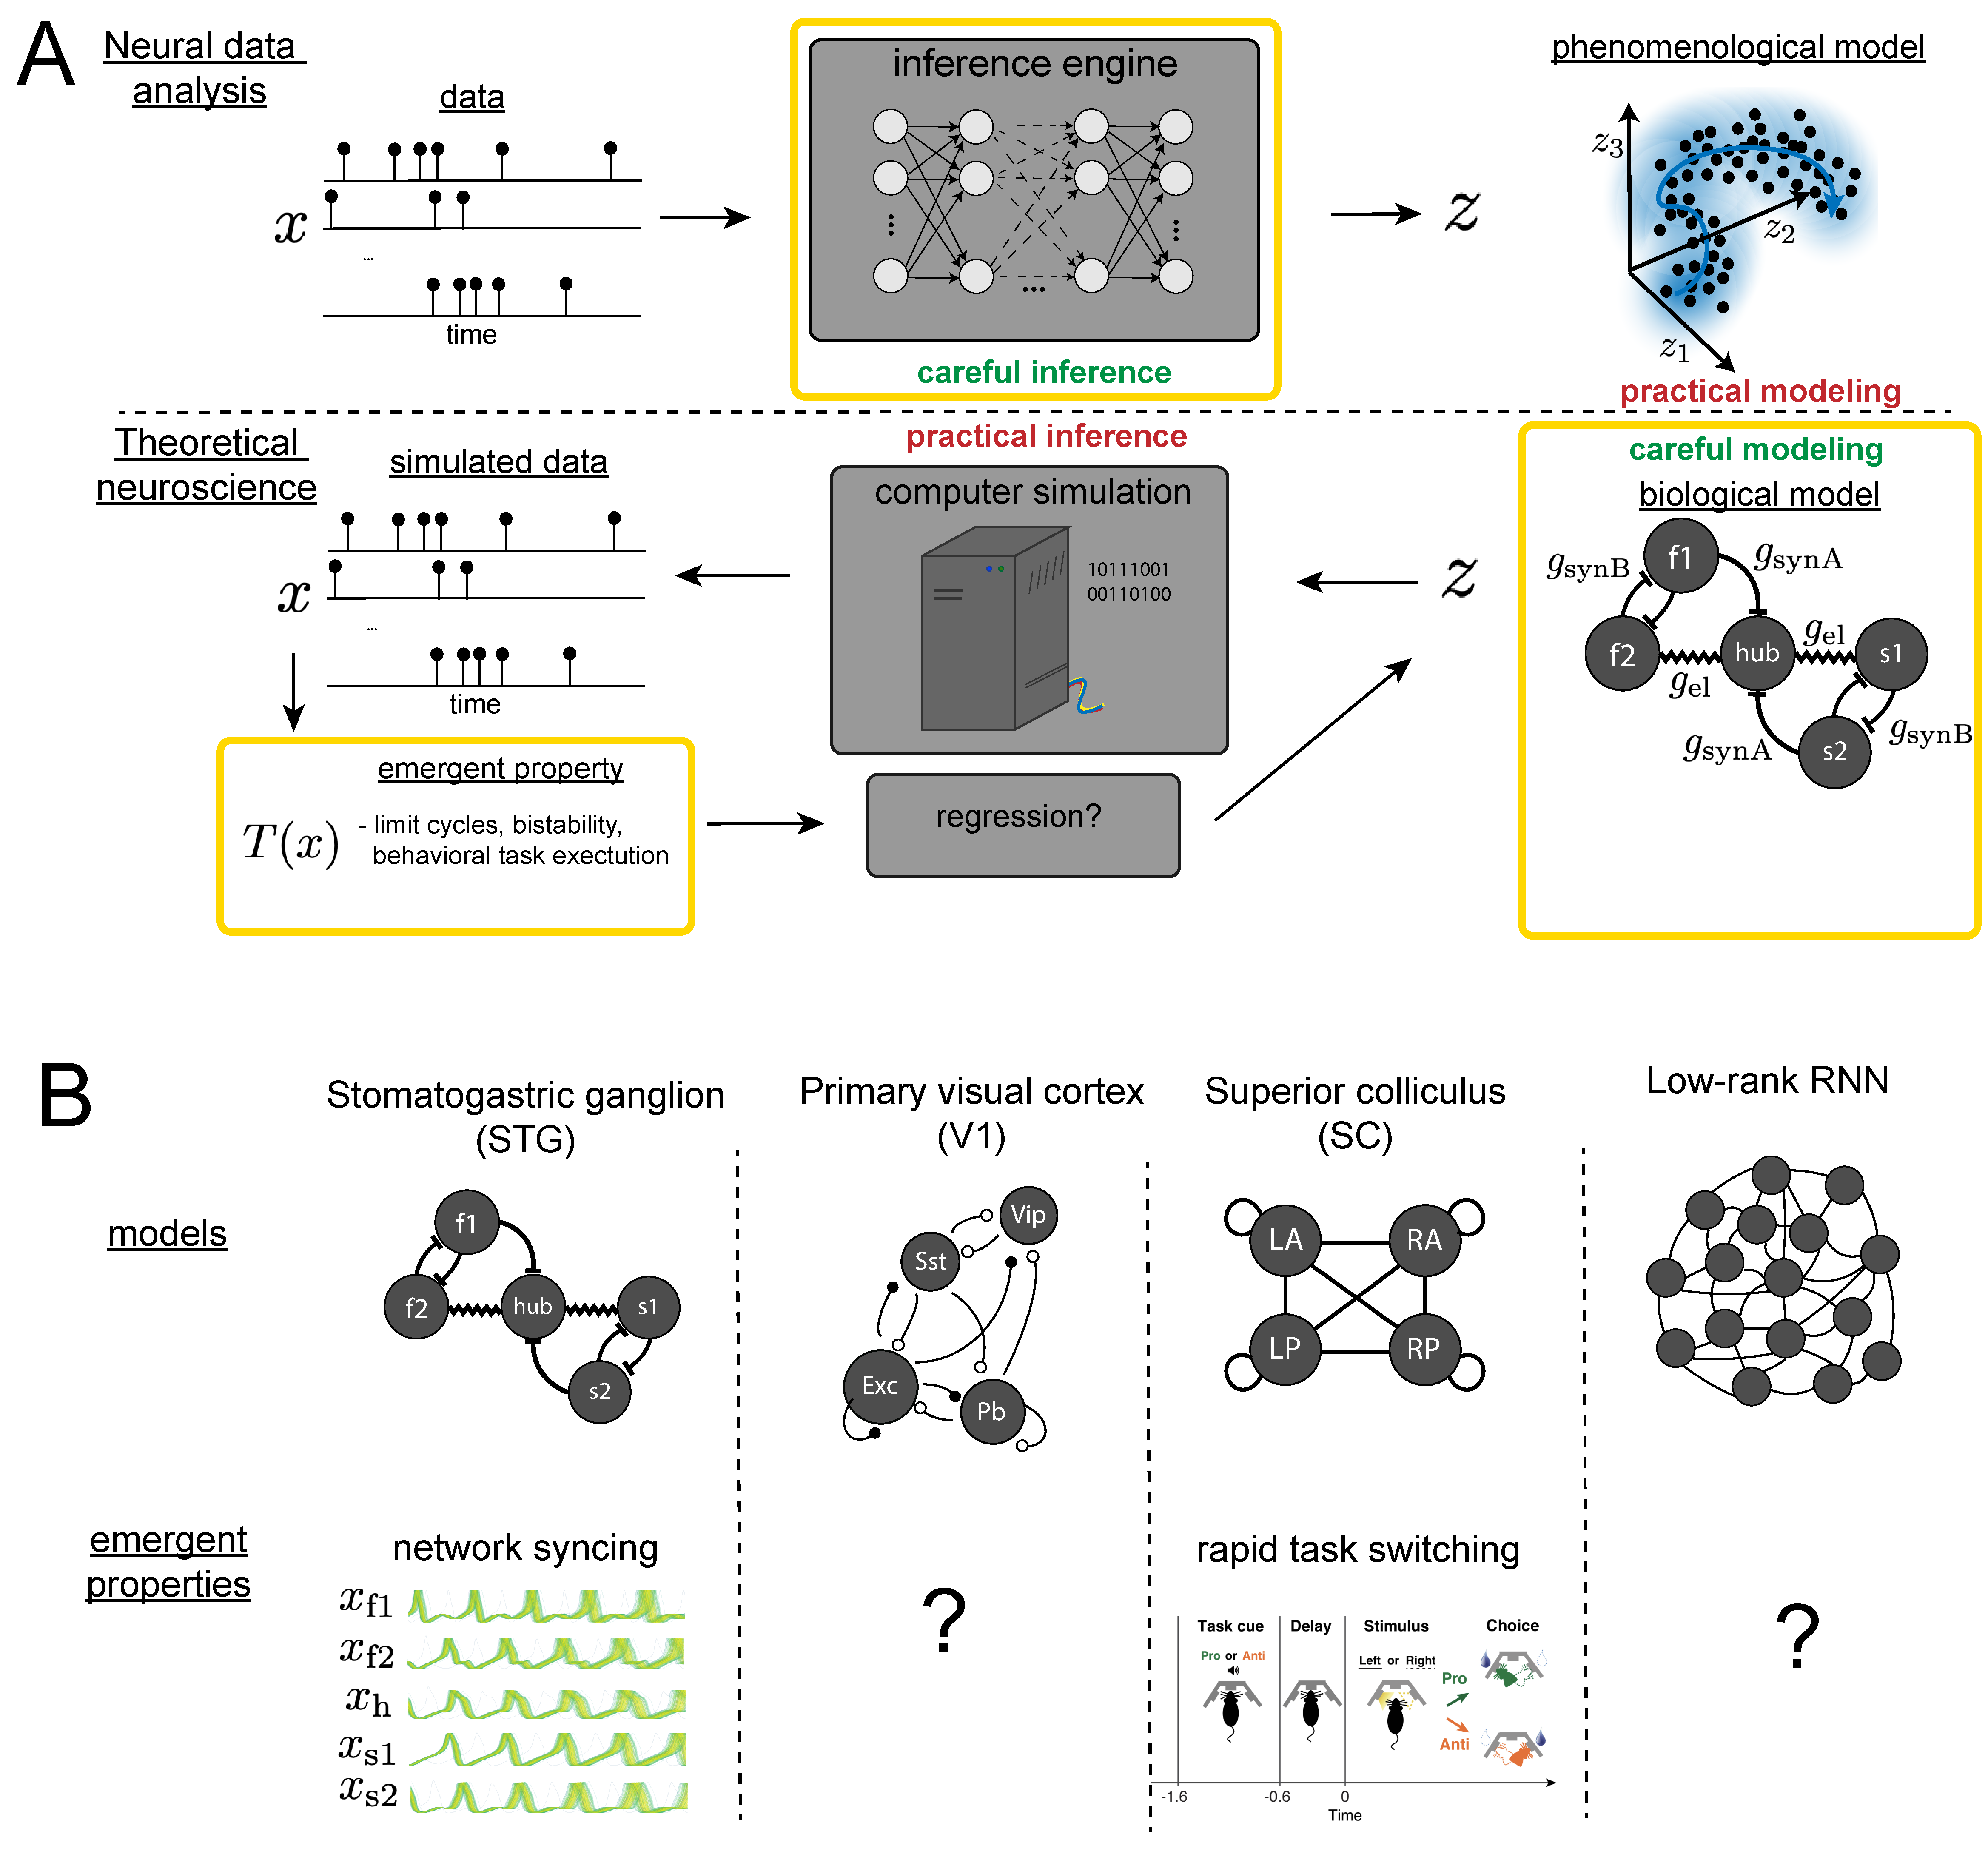
\includegraphics[scale=0.2]{figs/fig1/fig1.pdf}
\end{center}
\caption{\small A. \textit{Neural data analysis}: To identify structure in experimentally recorded neural data sets (left), neural data analysts use the modern inference engine (center) -- a collection of tools like convex optimization theory and deep learning from the machine learning literature -- to carefully execute Bayesian inference on a phenomenological generative model of the data.  Neural data analysts impose practical constraints to these phenomenological models so that Bayesian inference can be done. \textit{Theoretical Neuroscience}: Theoretical neuroscientists design systems of equations reflecting biological reality comprising a model (right, e.g. the STG) with the hopes of reproducing emergent properties of neural computation found in data (left).  In standard practice, models are evaluated by simulating them for many choices of parameters on a server (center).  To gain an understanding for how parameters of the model govern such emergent properties, theoretical neuroscientists are left to measure correlations or find other structure in the simulated activity. In this study, we introduce DSNs, which use the modern inference engine to learn distributions of model solutions given emergent properties of neural computations (yellow boxes).  B. We use DSNs to provide novel insights to popular models in theoretical neuroscience.  We examine network syncing in the STG, blah in a dynamic four neuron-type population model of primary visual cortex (V1), information routing in the superior colliculus (SC), and blah in low-rank recurrent neural networks (RNNs).}
\end{figure}


Advancements in probabilistic machine learning have led to transformative changes in industrial applications like image processing (sparse cite), speech recognition (sparse cite), text classification (sparse cite), and more.  We call the generalizable components of this groundbreaking technology (deep learning, stochastic gradient descent, GPU parallelization, etc.) the ``modern inference engine." (Point to work from Cunningham/Paninski using modern inference engine for neuroscientific phenomenological models (PfLDS, BehaveNET)?) In this study, we use the modern inference engine to bypass the perceived intractability of statistical inference in realistic models of neural systems.  (Introduce SDNs?)  We demonstrate the widespread applicability of this approach by producing novel insights into network syncing in the stomatogastric ganglion (STG), neuron-type input-responsivity in primary visual cortex (V1), rapid task switching in superior colliculus (SC), and approximate Bayesian inference in recurrent neural networks (RNNs). \\

\section{Results}
\subsection{Degenerate solution networks}
\begin{itemize}
\item To translate progress in neural data analysis to theoretical neuro, need to key steps.
\begin{itemize}
\item 1. Need to learn parameter distributions of biologically realistic (not just phenom.) models.
\item 2. Must be able to condition on emergent properties of interest, not simply computationally convenient sufficient statistics of data sets.
\end{itemize}
\item Bayesian data scientists will say experimental data is all that matters.  
\item \textit{Transition}: This is untrue when working in a creative, exploratory modeling setting.
\end{itemize}

\textbf{Edgy contrarian point about theorists and data}
\begin{itemize}
\item Common misconception: theoreticians rarely attempt to directly reproduce experimental data. 
\item Instead, they work with (abstracted?) mathematical definitions of emergent properties.  
\end{itemize}

\textbf{DSNs}
\begin{itemize}
\item We introduce DSNs, which bridge methodology in these subfields of comp neuro.
\item  Combine ideas from MEFNs (cite Gabe) and LFVI (cite Dustin) to learn a deep probability distribution of theoretical model parameterizations $z$ that produce the emergent properties of interest $T(x)$ (see Appendix).  
\item Explain deep probability distributions.
\item DSNs are deep probability distributions of theoretical model parameters, which are optimized to be maximally random (maximum entropy) while producing the specified value of emergent properties:
\begin{equation}
\begin{split}
q_\theta^*(z) &= \argmax_{q_\theta \in Q} H(q_\theta(z)) \\
 &  \text{s.t.  } E_{z \sim q_\theta}\left[ E_{x\sim p(x \mid z)}\left[T(x)\right] \right] = \mu \\
 \end{split}
\end{equation}
\end{itemize}

\begin{figure}
\begin{center}
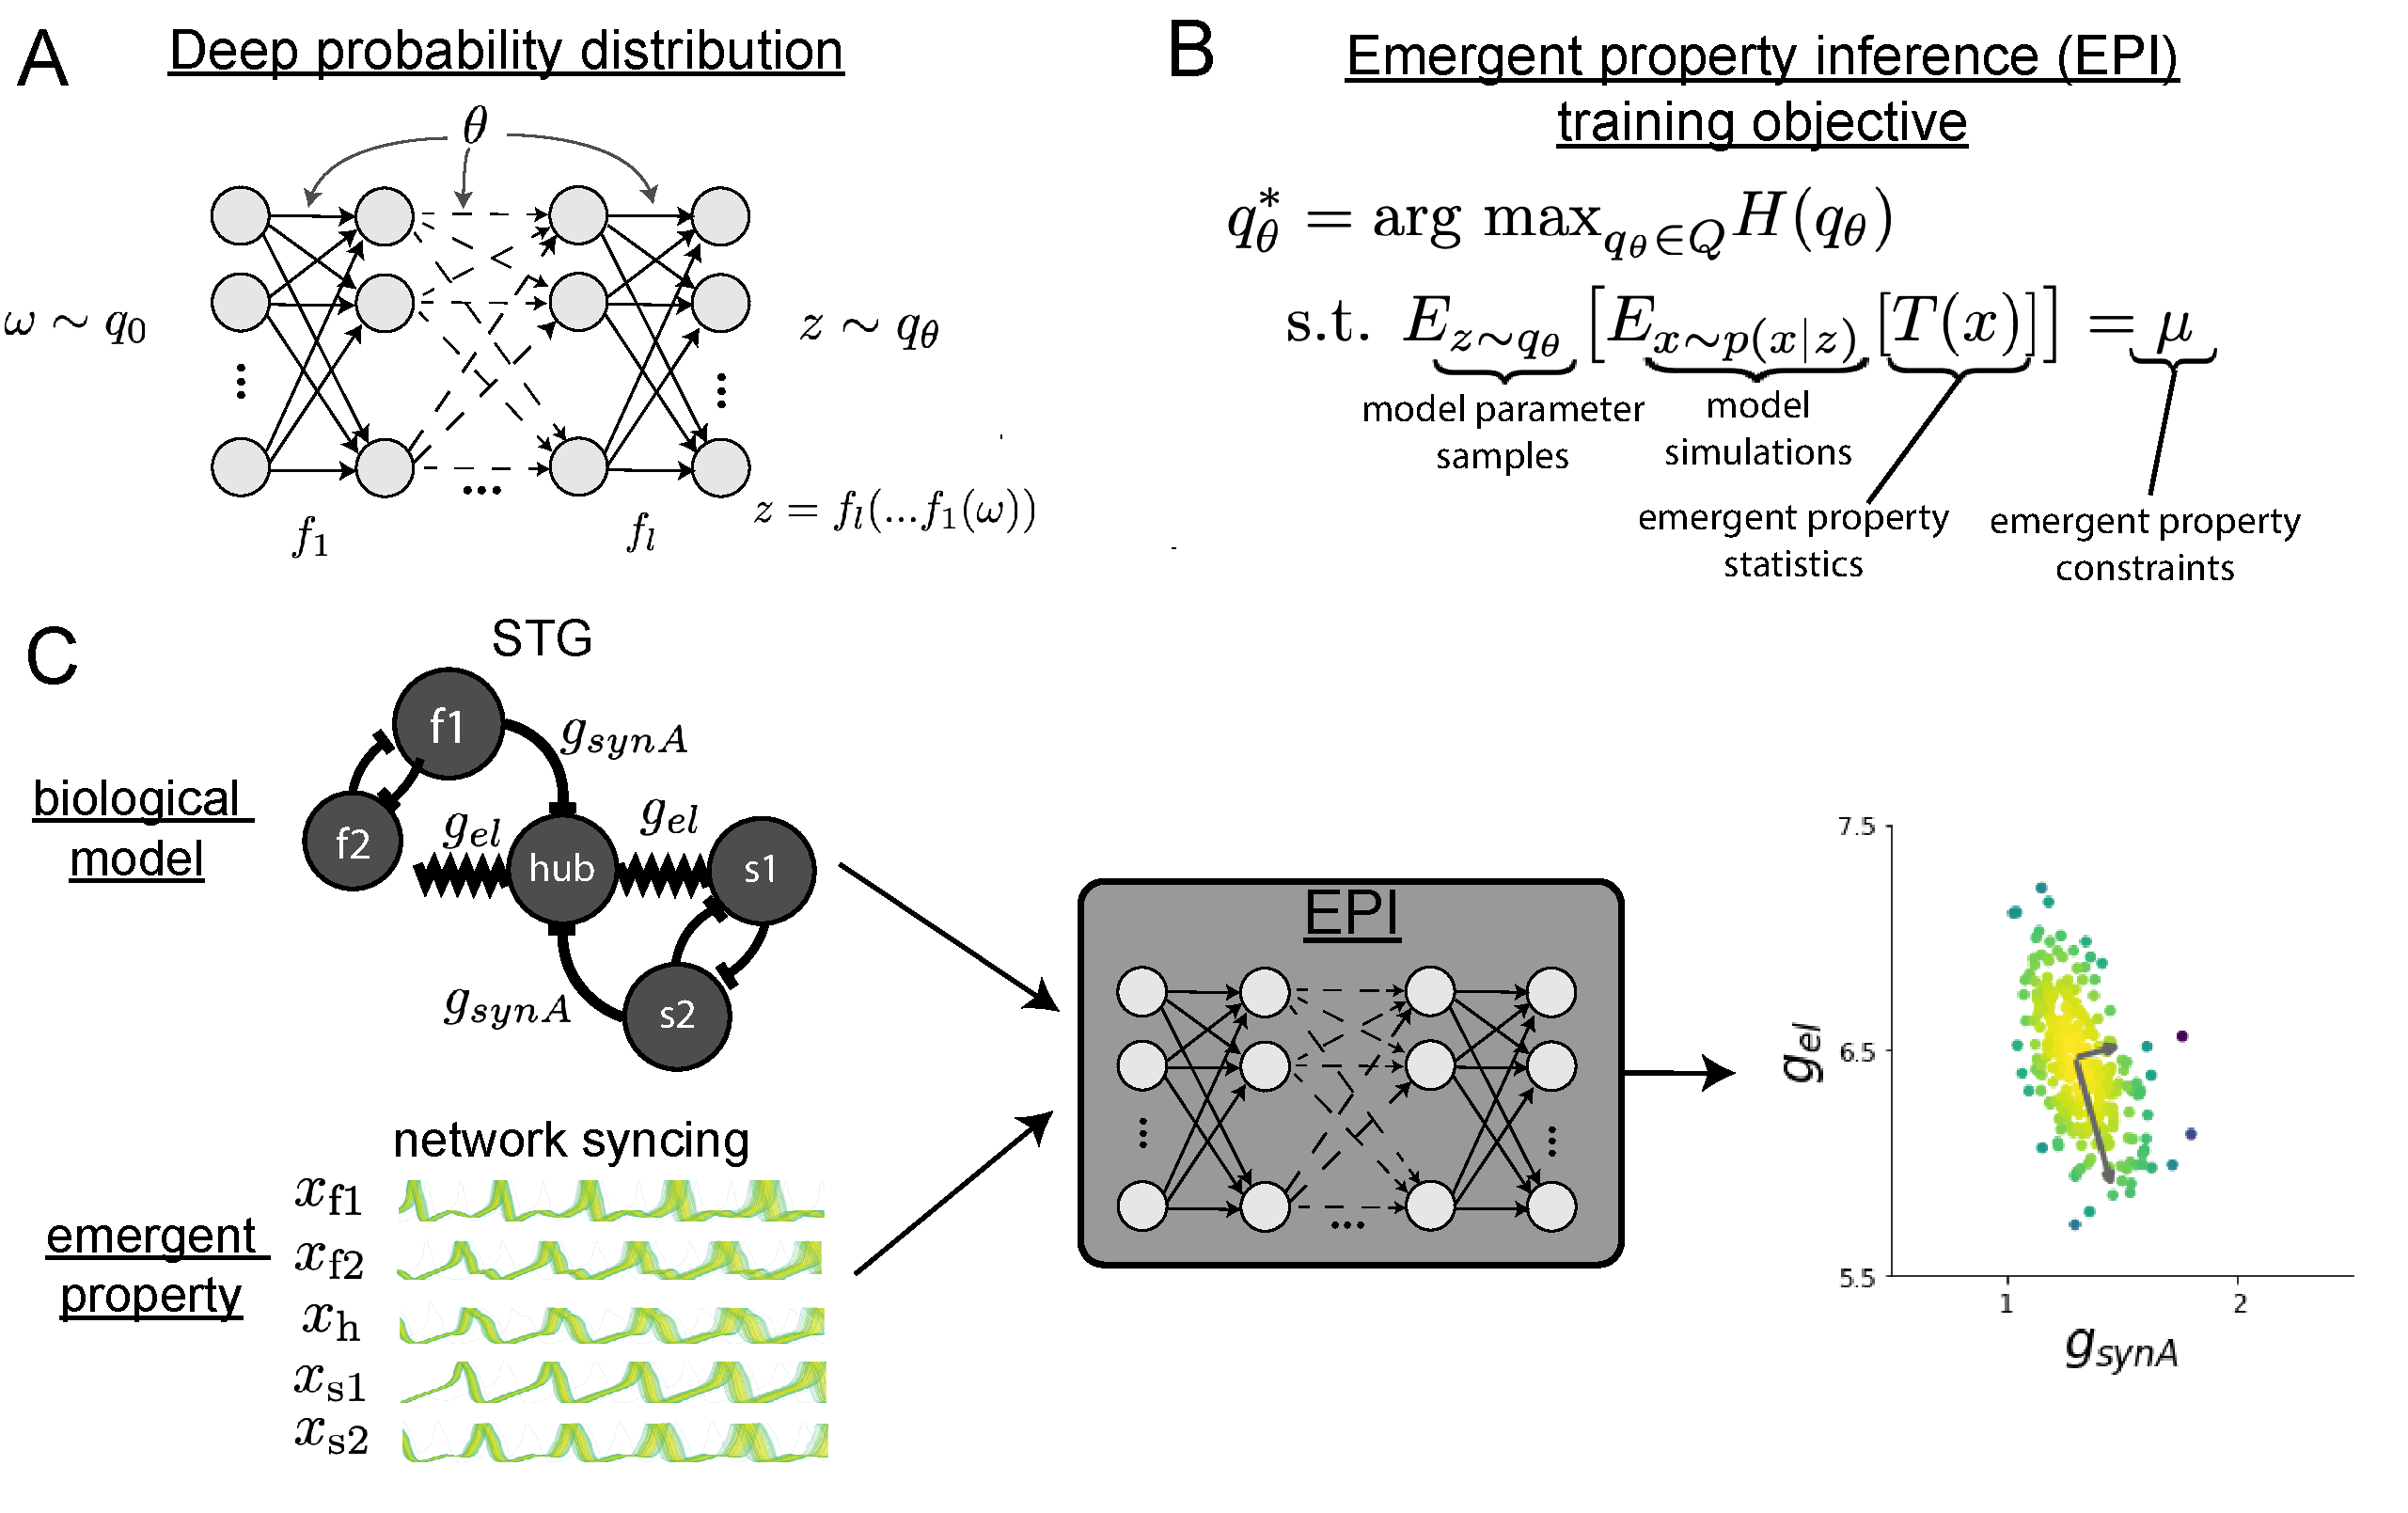
\includegraphics[scale=0.4]{figs/fig2/fig2.pdf}
\end{center}
\caption{A. Degenerate solution networks (DSNs) are deep probability distributions $q_\theta(z)$ of theoretical model parameterizations that produce emergent properties of interest.  The stochasticity of a deep probability distribution comes from a simple random variable $\omega \sim q_0$, where $q_0$ is often chosen to be an isotropic gaussian, and the structure comes from the deterministic transformation made by the deep neural network with optimized parameters $\theta$.  DSNs are the result of a constrained stochastic optimization, in which emergent properties $T(x)$ are fixed in expectation over model simulations $x \sim p(x \mid z)$ and DSN samples $z \sim q_\theta(z)$ to be a particular value $\mu$.  DSNs distributions maximize randomness through entropy. B. For a choice of model (STG) and emergent property (network syncing), a DSN learns a posterior distribution of the model parameters  $z = \left[g_{\text{el}}, g_{\text{synA}} \right]^\top$ conditioned on network syncing.}
\textbf{SB Comment}: In A, we have gaussian noise being fed into the deep probability distribution, and in B, we have a choice of model and emergent property predicating what the DSN is going to do.  There should be a way to depict these ideas without creating confusion on what the input to the DSN is.
\end{figure}

\textbf{Worked example: STG}
\begin{itemize}
\item For example, consider the STG.
\item Explain this STG circuit, emergent property of interest.
\item  For our choices of STG as model and network syncing as emergent property, we use a DSN to learn a distribution on STG conductance parameters that produces network syncing.  
\item Emphasize utility of DSN using Hessian.
\item An equivalent conceptualization is that DSNs do Bayesian inference (see Appendix).
\item Punchline about DSNs and transition to V1.
\end{itemize}

\subsection{Exploratory analysis of a theoretical model}
Will focus on this once result finalized.  Have a lot of text to pull from.

\subsection{Identifying sufficient mechanisms of task learning}
Will focus on this once V1 and LRRNN finalized.  Have a lot of text to pull from.

\subsection{Conditioning on computation with interpretable models of RNNs}
Will focus on this once result finalized.  Have a lot of text to pull from.

\section{Discussion}
\begin{itemize}
\item Summarize the key methodlogical demonstrations from the results section.
\item Talk big picture: If we know we can't analytically derive these things, we need an alternative characterization.  Simulate and examine isn't cutting it.  We need to be leveraging the modern inference engine to gain this understanding.  Bayesian probability is the framework we should use for this formalism.
\item Expand on idea of posterior predictive checks / hypothesis testing / exploratory analyses of models themselves.  Give the whole, we don't even understand the models we're developing pitch.
\item Elaborate on idea of conditioning on flexibly defined statistics i.e. emergent properties. Emphasize how this is practical.  Link to sufficient statistics, esp. commonly used in phenom models like spike counts etc.
\item Summarize the respective strengths SNPE and DSN.
\item Link conditioning on task execution with work done today with RNNs.  Basically, we're training overparameterized models with regression, and get a distribution (we have no prob treatment of). Emphasize utility of low-dim interpretable parameterizations.
\item A paragraph on bridging large scale recordings with theory.
\end{itemize}

\appendix

\section{Supplement}

\subsection{Models}
Here I'll explain all the models that we looked at.

\subsubsection{Stomatogastric ganglion}

\subsubsection{Primary visual cortex}
Dynamical models with two populations (excitatory (E) and inhibitory (I) neurons) of visual processing have been used to reproduce a host of experimentally documented phenomena in V1.  In particular regimes of excitation and inhbition, these models exhibit the paradoxical effect \cite{tsodyks1997paradoxical}, selective amplification \cite{murphy2009balanced}, surround suppression \cite{ozeki2009inhibitory}, and  sensory integrative properties \cite{rubin2015stabilized}.  Since I neurons mostly fall into one of three classes (parvalbumin (P)-, somatostatin (S)-, and vasointestinal peptide (V)-expressing neurons) \cite{markram2004interneurons, rudy2011three}, theorists look to extend these dynamical models to four populations \cite{litwin2016inhibitory}.  A current challenge in theoretical neuroscience is understanding the distributed role of inhibition stabilization across these subtypes.  

The dynamics of each neural populations average rate
$x = \begin{bmatrix} x_E \\ x_P \\ x_S \\ x_V \end{bmatrix}$
are given by:
\begin{equation}
\tau \frac{dx}{dt} = -x + [W x+ h]_+^n
\end{equation}

In some cases, these neuron types do not send projections to one of the other types \cite{pfeffer2013inhibition}.  Estimates of the of the probability of connection and strength of connection from the Allen institute result in an estimate of $W$ of 
\begin{equation}
W = \begin{bmatrix} 0.0576 &  0.19728 & 0.13144 & 0 \\
                                0.58855 & 0.30668 & 0.4285 & 0 \\
                                0.15652 & 0 & 0 & 0.2 \\
                                0.13755 & 0.0902 &  0.4004 &  0 \end{bmatrix}
\end{equation}

[Establish that we care about what inputs to this system make each neuron type respond at a fixed point.]  Sound analytic derivations can give us the linear approximation to the response, which is valuable close to the fixed point.  We can describe the dynamics of this system more generally by
\begin{equation}
\dot{x}_i = -x_i + f(u_i)
\end{equation}
where the input to each neuron is
\begin{equation}
u_i = \sum_j W_{ij} x_j + h_i
\end{equation}
Let $F_{ij} = \gamma_i \delta(i,j)$, where $\gamma_i = f'(u_i)$.  Then, the linear response is
\begin{equation}
\frac{\partial x}{\partial h} = F(W\frac{\partial x}{\partial h} + I)
\end{equation}
which is calculable by
\begin{equation}
\frac{\partial x}{\partial h} = (F^{-1} - W)^{-1}
\end{equation}

However, as we get further away from the fixed point, the linear approximation to the system response becomes less accurate.

We compare this linear prediction to the DSN distribution of inputs resulting in a given increase in neuron type population firing rate.

We measure this increase by simulating the system at $b = \begin{bmatrix} 1,1,1,1 \end{bmatrix}^\top$ and $b + dh$, for T=100 time steps using Euler intergration with $dt = 5$ms and $\tau = 20$ms, where we initialize the system to $x(0)_i \sim \mathcal{N}(1, 0.01)$.



\subsubsection{Superior colliculus}
There are four total units: two in each hemisphere corresponding to the PRO/CONTRA and ANTI/IPSI populations.  Each unit has an activity ($x_i$) and internal variable ($u_i$) related by
\begin{equation}
x_i(t) =\psi(t)\left(\frac{1}{2}\tanh\left(\frac{u_i(t) - \epsilon}{\zeta}\right)+ \frac{1}{2} \right)
\end{equation}
$\epsilon = 0.05$ and $\zeta = 0.5$ control the position and shape of the nonlinearity, repsectively, and $\psi(t)$ is the optogenetic inactivation function.

We can order the elements of $x_i$ and $u_i$ into vectors $x$ and $u$ with elements
\begin{equation}
x = \begin{bmatrix} x_{LP} \\ x_{LA} \\ x_{RP} \\ x_{RA} \end{bmatrix} \hspace{2cm} u = \begin{bmatrix} u_{LP} \\ u_{LA} \\ u_{RP} \\ u_{RA} \end{bmatrix}
\end{equation}

 The internal variables follow dynamics:
\begin{equation}
\tau \frac{\partial u}{\partial t} = -u + Wx + h + \sigma \partial B
\end{equation}
with time constant $\tau = 0.09s$ and gaussian noise $\sigma \partial B$ controlled by the magnitude of $\sigma$.  The weight matrix has 8 parameters $sW_P$, $sW_A$, $vW_{PA}$, $vW_{AP}$, $hW_P$, $hW_A$, $dW_{PA}$, and $dW_{AP}$,  related to the depiction in Fig. 2:
\begin{equation}
W = \begin{bmatrix} sW_P & vW_{PA} & hW_P & dW_{PA}  \\ vW_{AP}  & sW_A & dW_{AP}  & hW_A \\ hW_P & dW_{PA}  & sW_P & vW_{PA}  \\ dW_{AP}  & hW_A & vW_{AP}  & sW_A \end{bmatrix}
\end{equation}

\begin{equation}
h = h_{\text{constant}} + h_{\text{pro-bias}} + h_{\text{rule}} + h_{\text{choice-period}} + h_{\text{light}}
\end{equation}


\begin{equation} h_{\text{constant}}(t) = I_{\text{constant}} \begin{bmatrix} 1 & 1 & 1 & 1 \end{bmatrix}^\top 
\end{equation}
\begin{equation} h_{\text{P,bias}}(t) = I_{\text{P,bias}} \begin{bmatrix} 1 & 0 & 0 & 1 \end{bmatrix}^\top 
\end{equation}
\begin{equation}h_{\text{P,rule}}(t) = \begin{cases}
                           I_{\text{P,rule}} \begin{bmatrix} 1 & 0 & 0 & 1 \end{bmatrix}^\top,& \text{if } t\leq 1.2s \\
                            0,              & \text{otherwise}
                         \end{cases}
\end{equation}
\begin{equation} h_{\text{A,rule}}(t) = \begin{cases}
                           I_{\text{A,rule}} \begin{bmatrix} 0 & 1 & 1 & 0 \end{bmatrix}^\top,& \text{if } t\leq 1.2s \\
                            0,              & \text{otherwise}
                         \end{cases}
\end{equation}
\begin{equation} h_{\text{choice}}(t) = \begin{cases}
                           I_{\text{choice}} \begin{bmatrix} 1 & 1 & 1 & 1 \end{bmatrix}^\top,& \text{if } t > 1.2s \\
                            0,              & \text{otherwise}
                         \end{cases}
\end{equation}
                         
\begin{equation}  h_{\text{light}}(t) = \begin{cases}
                           I_{\text{light}} \begin{bmatrix} 1 & 1 & 0 & 0 \end{bmatrix}^\top,& \text{if } t > 1.2s \text{ and Left} \\
                           I_{\text{light}} \begin{bmatrix} 0 & 0 & 1 & 1 \end{bmatrix}^\top,& \text{if } t > 1.2s \text{ and Right} \\
                            0,              & t \leq 1.2s
                         \end{cases} 
\end{equation}

Let's say that we want to learn the parameters that produce a Bernoulli rate of $p_{LP}$ in the Left, Pro condition.  (We can generalize this to either cue, or stimulus condition).  We'll let $\hat{p}_i$ be the empirical average steady state (ss) response (final $V_{LP}$ at end of task) over M=100 gaussian noise draws for a given SC model parameterization $z_i$:

\begin{equation}
 \hat{p}_i = E_{\sigma \partial B} \left[ x_{LP,\text{ss}} \mid s=L, c=P, z_i \right] = \frac{1}{M}\sum_{j=1}^M x_{LP,\text{ss}}(s=L, c=P, z_i, \sigma \partial B_j)
 \end{equation}

The noise is fixed at $\sigma = 0.3$ (the average of satisfactory parameterizations from Duan et al.).  For the 1st constraint, we certainly want the average over DSN samples (from $q_\phi(z)$) to be $p_{LP}$:
\begin{equation}
E_{z_i \sim q_\phi} \left[ E_{\sigma \partial B} \left[ x_{LP,\text{ss}} \mid s=L, c=P, z_i \right] \right] = E_{z_i \sim q_\phi} \left[ \hat{p}_i \right] = p_{LP}
\end{equation}

We can then ask that the variance of the steady state responses across gaussian draws, is the Bernoulli variance for the empirical rate $\hat{p}$.
\begin{equation}
 Var_{\sigma \partial B} \left[ x_{LP,\text{ss}} \mid s=L, c=P, z_i \right] = \hat{p}_i(1 - \hat{p}_i)
\end{equation}

With DSNs, we enforce constraints in expectation over DSN samples, so we can force Bernoulli responses with this 2nd constraint:
\begin{equation}
E_{z \sim q\phi} \left[ Var_{\sigma \partial B} \left[ x_{LP,\text{ss}} \mid s=L, c=P, z_i \right] - \hat{p}_i(1 - \hat{p}_i) \right] = 0
\end{equation}

Since the maximum variance of a random variable bounded from 0 to 1 is the Bernoulli variance ($\hat{p}(1-\hat{p})$), in principle, we do not need to control the second moment (over DSN samples) of this test-static (the variance over gaussian draws).  In reality, these variables are dynamical system states and can only exponentially decay (or saturate) to 0 (or 1), so the Bernoulli variance constraint can only be undershot.  This is important to be mindful of when evaluating the convergence criteria.

We have an additional constraint that the Pro neuron on the opposite hemisphere should have the opposite value.  We can enforce this with a final constraint:
\begin{equation}
E_{z \sim q\phi} \left[ E_{\sigma \partial W} \left[ (x_{LP,\text{ss}} - x_{RP,\text{ss}})^2  \mid s=L, c=P, z_i \right] \right] = 0
\end{equation}

Training DSNs to learn distributions of dynamical system parameterizations that produce Bernoulli responses at a given rate (with small variance around that rate) was harder to do than expected.  Long story short: there is a pathology in this optimization setup, where the learned distribution of weights is bimodal attributing a fraction $p$ of the samples to an expansive mode (which always sends $x_{LP}$ to 1), and a fraction $1-p$ to a decaying mode (which always sends $x_{LP}$ to 0).  This pathology was avoided using an inequality constraint prohibiting parameter samples that resulted in low variance of responses across noise.

\subsubsection{Rank-1 RNN}



\subsection{Supplementary Figures}

\begin{figure}
\begin{center}
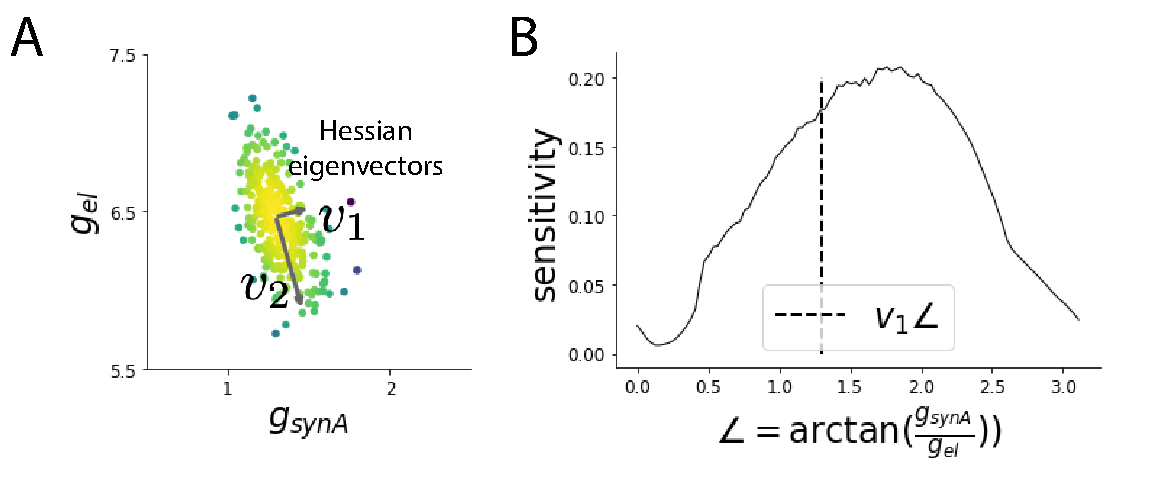
\includegraphics[scale=0.7]{figs/figS1/figS1.pdf}
\end{center}
Fig. S1: A. DSN distribution of STG model parameters producing network syncing.  B. Sensitivity of the system with respect to network syncing along all dimensions of parameter space away from the mode.
\end{figure}

\begin{figure}
\begin{center}
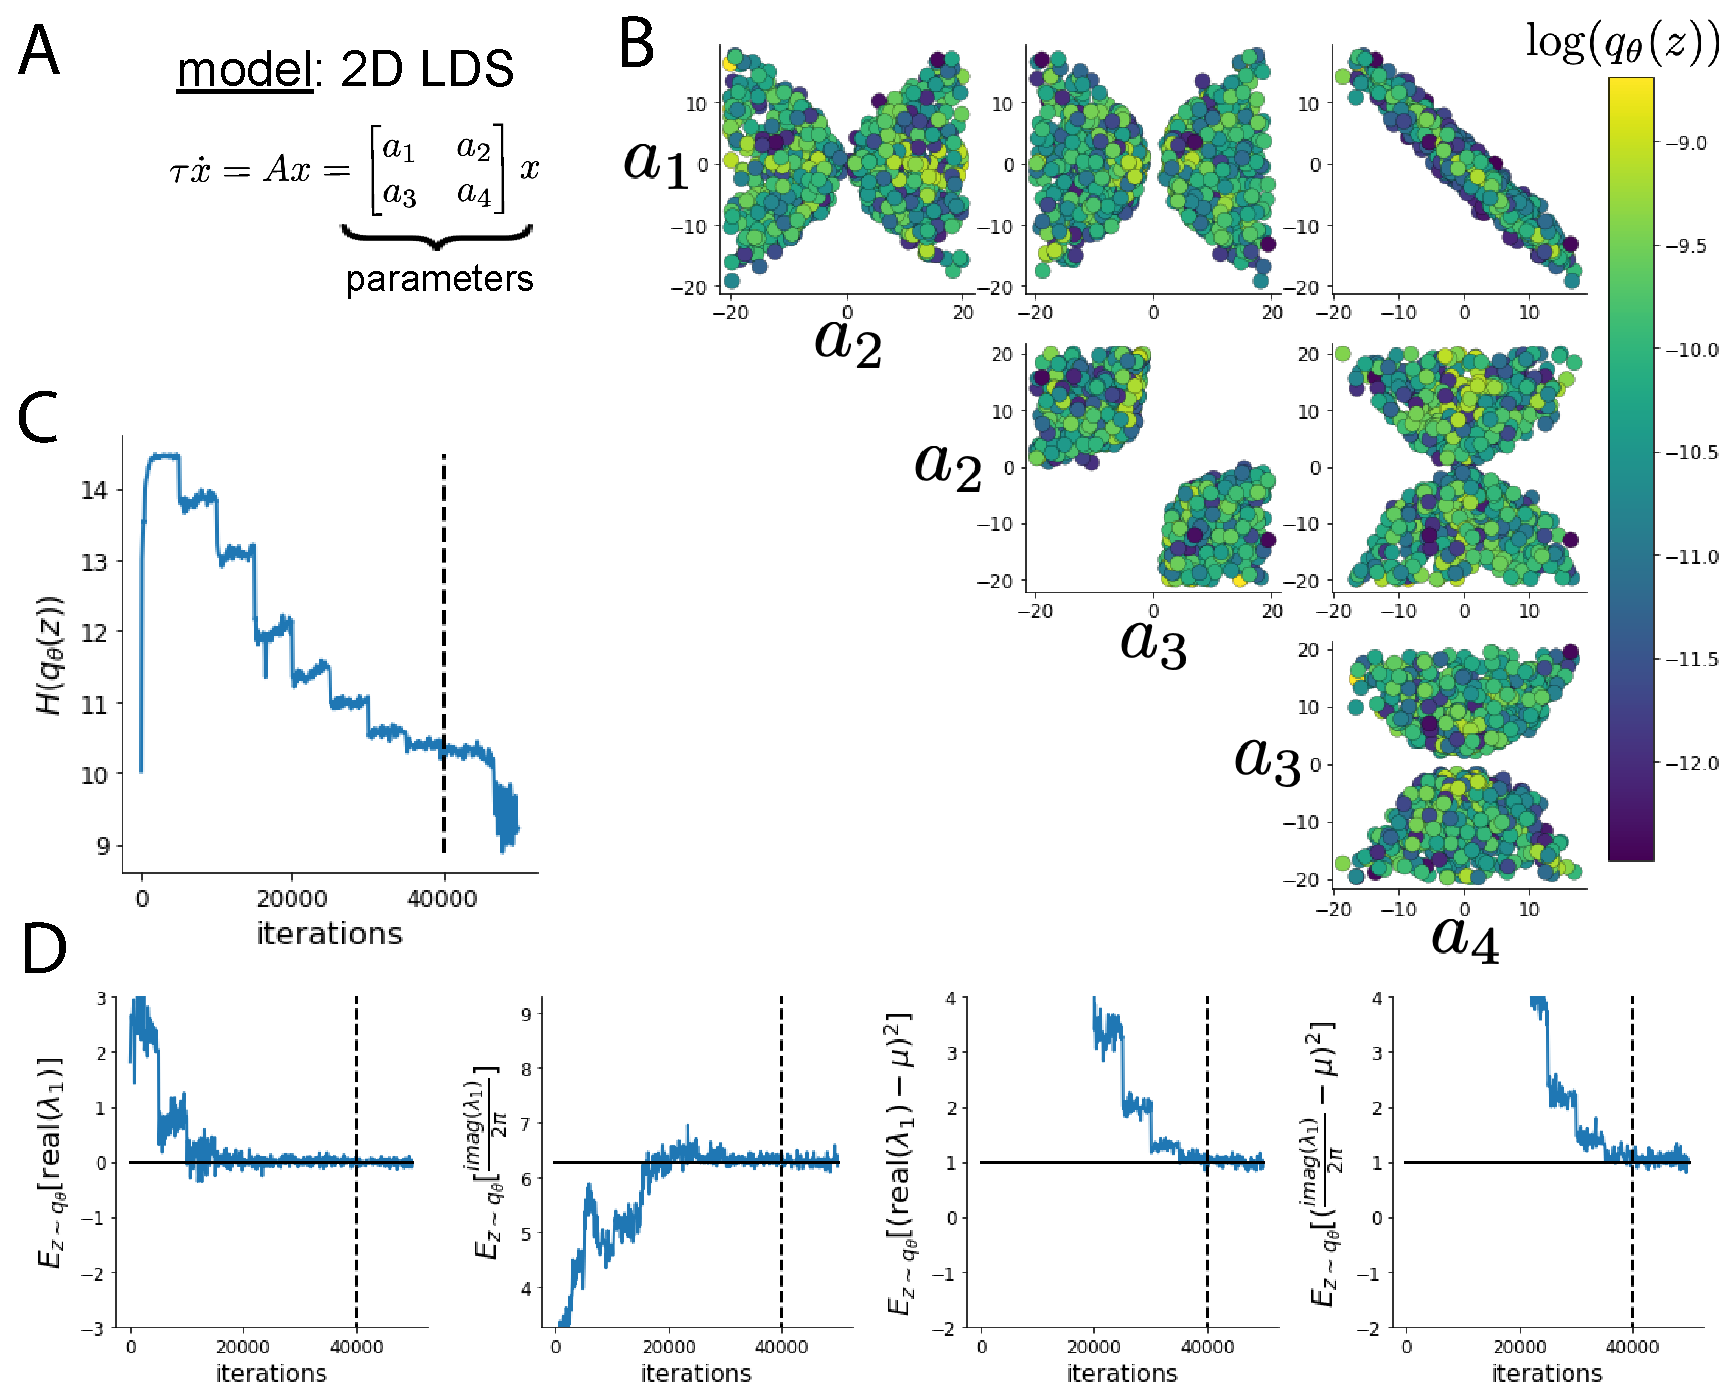
\includegraphics[scale=0.5]{figs/figS2/figS2.pdf}
\end{center}
Fig. S2: A. Two-dimensional linear dynamical system model, where real entries of the dynamics matrix $A$ are the parameters.  B. The DSN distribution for a 2D LDS with $\tau=1$ that produces an average of 1Hz oscillations with some small amount of variance.  C. Entropy throughout the optimization.  At the beginning of each augmented lagrangian epoch (5,000 iterations), the entropy dips due to the shifted optimization manifold where emergent property constraint satisfaction is increasingly weighted.  D. Emergent property moments throughout optimization.  At the beginning of each augmented lagrangian epoch, the emergent property moments move closer to their constraints.
\end{figure}




\bibliography{NN2019}
\bibliographystyle{unsrt}

\end{document}


